\documentclass[mathserif, handout]{beamer}

\usepackage{url}
\usepackage{longtable}
% ======================================================================
% General LaTeX Setup for Beamer (Reusable Preamble)
% Author: Chandra Gummaluru
% ======================================================================

\documentclass[mathserif, handout]{beamer}
\setbeamertemplate{frametitle}{}

% ------------------------------------------------------------
% basic packages
% ------------------------------------------------------------
\usepackage{url}
\usepackage{ifthen}
\usepackage{enumerate}
\usepackage[font=small]{caption}
\usepackage{subcaption}
\usepackage{moresize}
\usepackage[outline]{contour}
\usepackage{transparent}
\usepackage{worldflags}
\usepackage{bm}
\usepackage{graphbox}
\usepackage{mathtools}
\usepackage{multirow}
\usepackage{fontawesome5}
\usepackage{pifont}
\usepackage{array}
\usepackage{comment}

% ------------------------------------------------------------
% math
% ------------------------------------------------------------
\DeclarePairedDelimiter{\floor}{\lfloor}{\rfloor}
\DeclarePairedDelimiter{\ceil}{\lceil}{\rceil}

% ------------------------------------------------------------
% colors
% ------------------------------------------------------------
\definecolor{hl}{RGB}{248,196,69}
\definecolor{myred}{HTML}{ED5565}
\definecolor{myorange}{HTML}{FC6E51}
\definecolor{myyellow}{HTML}{FFCE54}
\definecolor{mycyan}{HTML}{4FC1E9}
\definecolor{myblue}{HTML}{5D9CEC}

\newcommand{\graytext}[1]{\footnotesize\color{gray}#1\normalsize\color{black}}

% ------------------------------------------------------------
% symbols
% ------------------------------------------------------------
\newcommand{\cmark}{\ding{51}}
\newcommand{\xmark}{\ding{55}}

% ------------------------------------------------------------
% highlighting
% ------------------------------------------------------------
\newcommand{\reducedstrut}{\vrule width 0pt height .9\ht\strutbox depth .9\dp\strutbox\relax}
\newcommand{\highlight}[1]{%
  \begingroup\setlength{\fboxsep}{0pt}\colorbox{hl}{\reducedstrut$\displaystyle #1$\/}\endgroup}
\newcommand{\highlightc}[2]{%
  \begingroup\setlength{\fboxsep}{0pt}\colorbox{#1}{\reducedstrut$\displaystyle #2$\/}\endgroup}

% ------------------------------------------------------------
% environments (boxes)
% ------------------------------------------------------------
\usepackage{tcolorbox}
\tcbuselibrary{skins}

\newtcolorbox{thmbox}[1][]{colback=gray!30!white!20, colframe=black, fonttitle=\bfseries, title=#1, boxrule=0.5pt}

% 1) Bottom open (draw top + sides only)
\newtcolorbox{thmboxtop}[1][]{
    enhanced,
    frame hidden,
    colback=gray!30!white!20,
    borderline north={0.5pt}{0pt}{black}, % top
    borderline west={0.5pt}{0pt}{black},  % left
    borderline east={0.5pt}{0pt}{black}   % right
}

% 2) Top open (draw bottom + sides only)
\newtcolorbox{thmboxbot}[1][]{
    enhanced,
    frame hidden,
    colback=gray!30!white!20,
    borderline south={0.5pt}{0pt}{black}, % bottom
    borderline west={0.5pt}{0pt}{black},  % left
    borderline east={0.5pt}{0pt}{black}   % right
}

% 3) Side only (draw only left and right)
\newtcolorbox{thmboxside}[1][]{
    enhanced,
    frame hidden,
    colback=gray!30!white!20,
    borderline west={0.5pt}{0pt}{black},  % left
    borderline east={0.5pt}{0pt}{black}   % right
}

\newtcolorbox{defboxtop}[1][]{
    enhanced,
    colback=gray!30!white!20,
    frame hidden,
    overlay={
        % Draw top + sides with rounded corners
        \draw[line width=0.5pt, black, rounded corners=3mm]
            (frame.south west) -- (frame.north west) -- (frame.north east) -- (frame.south east);
    },
    #1
}

\newtcolorbox{defboxbot}[1][]{
    enhanced,
    colback=gray!30!white!20,
    frame hidden,
    overlay={
        % Draw top + sides with rounded corners
        \draw[line width=0.5pt, black, rounded corners=3mm]
            (frame.north west) -- (frame.south west) -- (frame.south east) -- (frame.north east);
    },
    #1
}

\newtcolorbox{defboxside}[1][]{
    enhanced,
    frame hidden,
    colback=gray!30!white!20,
    borderline west={0.5pt}{0pt}{black},  % left
    borderline east={0.5pt}{0pt}{black}   % right
}

\newtcolorbox{proofbox}[1][]{colback=gray!20!white!20, colframe=grey, fonttitle=\bfseries, title=#1, boxrule=0.5pt, colbacktitle=white, enhanced jigsaw, sharp corners}

% ------------------------------------------------------------
% code listings
% ------------------------------------------------------------
\usepackage{listings}
\lstdefinestyle{mypython}{
  language=Python,
  deletekeywords=[2]{open, next, from, chr, str, int},
  morekeywords=[3]{List, Graph, Tree, Dict, Set, UnionFind, Ordict, Trie, Queue},
  morekeywords=[4]{ListNode, Vertex, Edge, Path, TreeNode, DictNode, UnifNode, OrdictNode, TrieNode, QueueNode},
  morekeywords=[5]{True, False, Boolean, String, Integer, Key, Function, KeyedObject, Object, Array, Tuple, Optional, None},
  keywordstyle=\color{mycyan}\bfseries,
  keywordstyle=[3]\color{myblue}\bfseries,
keywordstyle=[4]\color{myblue}\bfseries,
keywordstyle=[5]\color{mycyan}\bfseries,
  stringstyle=\color{orange},
  commentstyle=\color{gray}\itshape,
  basicstyle=\ttfamily\footnotesize,
  numbers=left,
  numberstyle=\tiny\color{gray},
  stepnumber=1,
  numbersep=5pt,
  xleftmargin=15pt,
  frame=none,
  showstringspaces=false,
  breaklines=true,
  breakatwhitespace=true,
  tabsize=4,
  columns=flexible
}


% ------------------------------------------------------------
% algorithms
% ------------------------------------------------------------
\usepackage{algorithm}
\usepackage[endLComment=~]{algpseudocodex}
\makeatletter
\algrenewcommand\ALG@beginalgorithmic{\footnotesize}
\makeatother

% ------------------------------------------------------------
% optimization environments
% ------------------------------------------------------------
\usepackage[nocomma]{optidef}

% ------------------------------------------------------------
% pgfplots and pie charts
% ------------------------------------------------------------
\usepackage{pgfplots}
\usepackage{pgf-pie}
\pgfplotsset{compat=1.7}

% ------------------------------------------------------------
% tikz
% ------------------------------------------------------------
\usepackage{tikz}
\usetikzlibrary{
  angles, quotes, positioning, fit, backgrounds, shapes.geometric, intersections,
  calc, shapes, mindmap, decorations.text, arrows, arrows.meta,
  automata, chains, decorations.pathreplacing, calligraphy,
  decorations.markings, shapes.misc, decorations.pathmorphing
}
\tikzset{
  invisible/.style={opacity=0},
  visible on/.style={alt=#1{}{invisible}},
  alt/.code args={<#1>#2#3}{\alt<#1>{\pgfprioritysalso{#2}}{\pgfprioritysalso{#3}}}
}

\newcommand{\multiedge}[5][]{
\pgfmathsetmacro{\N}{#4}
\pgfmathsetmacro{\mid}{(\N-1)/2}
\foreach \i in {0,...,\numexpr#4-1\relax} {

\pgfmathsetmacro{\k}{\i-\mid}
\draw[#1] ($ (#2) + \k*#5*($(#2)!1!90:(#3)$) $) -- ($ (#3) + \k*#5*($(#2)!1!90:(#3)$) $); 

}
\draw[#1,  -{>[scale=1]}]
  ($(#2)!0.54!(#3)$) -- ($(#2)!0.55!(#3)$);
}

% ------------------------------------------------------------
% bibliography
% ------------------------------------------------------------
\usepackage[style=ieee]{biblatex}
\setbeamertemplate{bibliography item}{\insertbiblabel}
\setbeamertemplate{background canvas}{
  \begin{tikzpicture}[remember picture,overlay]
    \node[opacity=0.0075]
      at (current page.center)
      {
\includegraphics[width=0.8\paperwidth]{images/signature.pdf}};
  \end{tikzpicture}
}

% ------------------------------------------------------------
% beamer theme and settings
% ------------------------------------------------------------
\usetheme{Boadilla}
\usecolortheme{seagull}
\beamertemplatenavigationsymbolsempty
\setbeamertemplate{enumerate item}{(\arabic{enumi})}
\setbeamertemplate{enumerate subitem}{(\alph{enumii})}
\setbeamertemplate{enumerate subsubitem}{(\roman{enumiii})}
\setbeamertemplate{itemize item}[circle]
\setbeamertemplate{itemize subitem}{\circ}
\setbeamertemplate{itemize subsubitem}{-}
\setbeamercolor{item}{fg=black!40}
\setbeamercovered{transparent=10}

% ===========================
% Premade TikZ Figure Commands
% ===========================

% images w/ labels
% inside tikz as a node
\NewDocumentCommand{\labeledimgnodetikz}{O{} m m m m m m}{%
	\begin{scope}[transparency group, #1]
		\node[
			draw,
			circle,
			inner sep=0,
			outer sep=0,
			minimum size=10mm,
			#1
		] (#5) at (#3,#4)
		{\includegraphics[scale=#7]{#6}};
		\node[
			rectangle,
			draw=black,
			thick,
			fill=black!55,
			rounded corners=0.1mm,
			inner sep=0pt,
			outer sep=0pt,
			minimum size=2.8mm,
			minimum width=3.5mm
		] at (#3,#4-0.1) {};
		\node[outer sep=0, inner sep=0, white] at (#3,#4-0.1) {\footnotesize #2};
	\end{scope}
}

% inside tikz isolated

% outside tikz
\NewDocumentCommand{\labelednode}{m}{%
	\begin{tikzpicture}[baseline={(0,-1mm)}]
		\node[
			rectangle,
			thick,
			draw=black,
			fill=black!55,
			rounded corners=0.1mm,
			inner sep=0pt,
			outer sep=0pt,
			minimum size=2.8mm,
			minimum width=3.5mm
		] at (0,0) {};
		\node[outer sep=0, inner sep=0, white, minimum size=2.8mm, minimum width=3.5mm] at (0,0) {\footnotesize #1};
	\end{tikzpicture}
}

% images only
% inside tikz as a node
\NewDocumentCommand{\imgnodetikz}{O{} m m m m m m}{%
	\begin{scope}[transparency group, #1]
		\node[
			draw,
			circle,
			inner sep=0,
			outer sep=0,
			minimum size=10mm,
			#1
		] (#5) at (#3,#4)
		{\includegraphics[scale=#7]{#6}};
		\node[
			rectangle,
			draw,
			thick,
			fill=black!55,
			rounded corners=0.1mm,
			inner sep=0pt,
			outer sep=0pt,
			minimum size=2.8mm,
			minimum width=3.5mm,
			opacity=0
		] at (0,0) {};
		\node[outer sep=0, inner sep=0, white, opacity=0] at (0,0) {\footnotesize #2};
	\end{scope}
}

% inside tikz isolated
\NewDocumentCommand{\imgtikz}{O{} mm}{%
	\begin{scope}[transparency group, #1]
		\node[
			inner sep=0,
			outer sep=0
		] (#5) at (#3,#4)
		{\includegraphics[scale=#3]{#2}};
	\end{scope}
}


% outside tikz
\NewDocumentCommand{\imgnode}{mm}{%
	\begin{tikzpicture}[baseline={(0,-1mm)}]
        \node[
            inner sep=0,
            outer sep=0,
            draw opacity=0,
        ] at (0,0)
        {\includegraphics[scale=#2]{#1}};
    \end{tikzpicture}
}

% outside tikz (inline)
\newcommand{\imgnodetext}[2]{%
	\hspace{-0.5mm}%
	\raisebox{-0.26\height}{%
		\includegraphics[scale=#2]{#1}%
	}%
	\hspace{-0.5mm}%
}


% labels only
% inside tikz as a node
\NewDocumentCommand{\labeltikz}{m}{%
	\node[
		rectangle,
		thick,
		draw=black,
		fill=black!55,
		rounded corners=0.1mm,
		inner sep=0pt,
		outer sep=0pt,
		minimum size=2.8mm,
		minimum width=3.5mm
	] at (0,0) {};
	\node[outer sep=0, inner sep=0, white, draw opacity=0] at (0,0) {\footnotesize #1};
}

% inside tikz isolated

% outside tikz

% === define custom pgfkeys ===
\pgfkeys{
	/devicenode/.is family, /devicenode,
	outline thickness/.initial=thick,
	outline color/.initial=black
}

\NewDocumentCommand{\qpacket}{m}{%
	\begin{tikzpicture}[baseline=(current bounding box.center)]
		\node at (0.5,0.4) {\includegraphics[scale=0.1]{#1}};
	\end{tikzpicture}%
}

\NewDocumentCommand{\bpacketid}{mmm}{%
	\begin{tikzpicture}[baseline=(current bounding box.center)]
		\begin{scope}[shift={(0.85,0.7)}]
			\draw[thick, draw=black, fill=#1, rounded corners=1pt] (0.01,0.05) rectangle node[white, text width=1cm, align=center] {\color{#3}\footnotesize #2} (-0.71,-0.625);
		\end{scope}
	\end{tikzpicture}%
}

\NewDocumentCommand{\packetid}{mmmm}{%
	\begin{tikzpicture}[baseline=(current bounding box.center)]
		\begin{scope}[shift={(0.85,0.7)}]
			\draw[thick, draw=black, fill=#2, rounded corners=1pt] (0.01,0.05) rectangle node[white, text width=1cm, align=center] {\color{#4}\footnotesize #3} (-0.71,-0.625);
			\node[
				star,
				star points=30,
				star point ratio=0,
				scale=1.5,
				draw=black,
				thick,
				fill=white,
				rounded corners=0.1mm,
				inner sep=0pt,
				minimum size=2.8mm
			] at (0,0) {};
			\node at (0,0) {\footnotesize #1};
		\end{scope}
	\end{tikzpicture}%
}

\tikzset{
	dictnode/.pic={
			\draw[thick, fill=#1, line join=]
			(-0.75,-0.5) --
			(-0.75,0.5)  --
			(0.75,0.5) --
			(0.75,-0.5) --
			cycle --
			(-0.75, 0.75) --
			(0.75, 0.75) --
			(0.75, -0.5) --
			cycle;
		}
}

\tikzset{
	queuenode/.pic={
			\draw[thick, fill=#1, line join=round]
			(-0.85,-0.5) --
			(-0.85,0.5)  --
			(0.65,0.5) --
			(0.75,0) --
			(0.65,-0.5) --
			cycle;
		}
}

\tikzset{
	queuenodetail/.pic={
			\draw[thick, fill=#1, line join=round]
			(-0.75,-0.5) --
			(-0.75,0.5)  --
			(0.65,0.5) --
			(0.75,0) --
			(0.65,-0.5) --
			cycle;
		}
}

\tikzset{
	listnode/.style={
			shape=rectangle,
			rounded corners,
			thick,
			minimum height=10mm,
			minimum width=15mm,
			inner sep=0pt
		}
}

\tikzset{
	arraynode/.style={
			shape=rectangle,
			thick,
			minimum height=10mm,
			minimum width=15mm,
			inner sep=0pt
		}
}

\tikzset{
	graphnode/.style={
			shape=circle,
			thick,
			minimum size=5mm,
			inner sep=0pt
		}
}

\tikzset{
	defaultnode/.style={
			transform shape,
			circle,
			draw=black,
			thick,
			fill=white,
			minimum size=10mm,
			inner sep=0pt
		},
	newnode/.style={
			transform shape,
			defaultnode,
			draw=myyellow,
			fill=myyellow!60,
			very thick
		},
	newnodelight/.style={
			transform shape,
			defaultnode,
			draw=myyellow,
			fill=myyellow!30,
			very thick
		},
	deletenode/.style={
			defaultnode,
			draw=gray,
			dashed,
			fill=lightgray,
			text=gray,
			very thick
		},
	nooutlinenode/.style={
			defaultnode,
			draw=none,
            draw opacity=0,
			text=black,
			very thick
		},
    nofillnode/.style={
			defaultnode,
			fill=none,
            text=black,
			very thick
		}
}
\tikzset{
	faded/.style={opacity=0.5, text opacity=0.5, transparency group}
}
\tikzset{
	smallgraytext/.style={font=\footnotesize\color{gray}}
}
\tikzset{
	graytext/.style={font=\normalsize\color{gray}}
}
\tikzset{
  squigglearrow/.style={
    very thick,
    lightgray,
    decorate,
    decoration={
      snake,
      amplitude=1.75pt,
      segment length=8pt
    }
  }
}



% title
\title{Epilogue}
\subtitle{Algorithms and Data Structures}
\author[C. Gummaluru]{Chandra Gummaluru}
\titlegraphic{
\includegraphics[width=0.15\linewidth]{images/signature.pdf}}
\institute[]{\url{chandra-gummaluru.github.io} }
\date[Algorithms and Data Structures]{}
\begin{document}

% beamer
\beamertemplatenavigationsymbolsempty
\setbeamertemplate{enumerate item}{(\arabic{enumi})}
\setbeamertemplate{enumerate subitem}{(\alph{enumii})}
\setbeamertemplate{enumerate subsubitem}{(\roman{enumiii})}

\setbeamertemplate{itemize item}[circle]
\setbeamertemplate{itemize subitem}{\circ}
\setbeamertemplate{itemize subsubitem}{-}
\setbeamercolor{item}{fg=black!40}

\setbeamercovered{transparent=10}

% pgfplots
\pgfplotsset{compat=1.7}

% tikz
\tikzset{
  invisible/.style={opacity=0},
  visible on/.style={alt=#1{}{invisible}},
  alt/.code args={<#1>#2#3}{%
      \alt<#1>{\pgfkeysalso{#2}}{\pgfkeysalso{#3}}
    },
}

\begin{frame}
  \maketitle
\end{frame}

\begin{frame}
  \begin{minipage}{0.5\textwidth}
    \centering
    \highlight{\textbf{algorithm}} \\[2mm]
    \graytext{a sequence of steps \\ to complete a task}
  \end{minipage}%
  \begin{minipage}{0.5\textwidth}
    \centering
    \highlight{\textbf{data structure}} \\[2mm]
    \graytext{an object used to hold data \\ written or read by algorithm}
  \end{minipage}
\end{frame}


\begin{frame}{Motivation}
  \begin{center}
    \Large \highlight{\textbf{motivation}}
  \end{center}
\end{frame}

\begin{frame}
  We want to design systems that allow devices to \highlight{\textbf{quickly}} and \highlight{\textbf{reliably}} communicate with each other.
  \begin{figure}
    \centering
    \begin{tikzpicture}
      \node at (4,0.7) {
\includegraphics[scale=0.13]{images/cloud.png}};

      \node (m1) at (0,0.5) {\includegraphics[scale=0.052]{images/server.png}};
      \node (m2) at (6.5,3) {
\includegraphics[scale=0.052]{images/phone.png}};
      \node (m3) at (7.5,-1) {\includegraphics[scale=0.052]{images/computer.png}};
      \node (m4) at (9.5,0.5) {
\includegraphics[scale=0.052]{images/router.png}};

      \draw[very thick, dashed] (m1) edge[bend left=10] (2.35,0.8);
      \draw[very thick, dashed] (m2) edge[bend right=10] (4.8,2.25);
      \draw[very thick, dashed] (m3) edge[bend right=10] (6.5, 0);
      \draw[very thick, dashed] (m4) edge[bend right=10] (6,0.7);
    \end{tikzpicture}
  \end{figure}
\end{frame}

\begin{frame}{Algorithms}
  \begin{center}
    \Large \highlight{\textbf{algorithms}}
  \end{center}
\end{frame}

\begin{frame}
  In solving our motivating problem, we studied these algorithms:\\[2mm]
  \begin{itemize}
    \item \highlight{\textbf{path-finding algorithms}}: \\
          \graytext{ used when a device needs to send a message efficiently to another device}
          \\[2mm]
    \item \highlight{\textbf{spanning tree algorithms}}: \\
          \graytext{ used when a device needs to broadcast a message efficiently to multiple devices}
          \\[2mm]
    \item \highlight{\textbf{sorting algorithms}}: \\
          \graytext{ used to ensure that messages with dependencies are sent in the correct order}
          \\[2mm]
    \item \highlight{\textbf{scheduling algorithms}}: \\
          \graytext{ used when a device must send multiple messages with timing constraints}

  \end{itemize}
\end{frame}

\begin{frame}
  We wanted our algorithms to satisfy the following properties: \\[2mm]
  \begin{itemize}
    \item \highlight{\textbf{halting}}:\\
          \graytext{ the algorithm always returns a (possibly \texttt{NULL}) solution}
          \\[2mm]
    \item \highlight{\textbf{complete}}:\\
          \graytext{ the algorithm returns a non-\texttt{NULL} solution whenever a non-\texttt{NULL} solution exists}
          \\[2mm]
    \item \highlight{\textbf{sound}}:\\
          \graytext{ the algorithm returns \texttt{NULL} whenever no solution exists}
          \\[2mm]
    \item \highlight{\textbf{optimal}}:\\
          \graytext{ the algorithm returns the optimal solution when multiple non-\texttt{NULL} solutions exist}
          \\[2mm]
    \item \highlight{\textbf{time-efficient}}:\\
          \graytext{ the algorithm requires minimal time}
          \\[2mm]
    \item \highlight{\textbf{space-efficient}}:\\
          \graytext{ the algorithm requires minimal memory}
  \end{itemize}
\end{frame}

\begin{frame}{Data Structures}
  \begin{center}
    \Large \highlight{\textbf{data structures}}
  \end{center}

\end{frame}

\begin{frame}
  To implement these algorithms and retain as many desired properties as possible, we also studied several supporting data structures:\\~\\
  \begin{itemize}
    \item[(1)] \highlight{\textbf{arrays}} \\
          \graytext{stores items in order} \\[3mm]
          \begin{figure}
            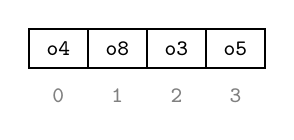
\begin{tikzpicture}

              \node[draw=white, text=black] (l1) at (0,-0.6) {\footnotesize\graytext{\texttt{0}}};
              \node[draw=white, text=black] (l2) at (0.75,-0.6) {\footnotesize\graytext{\texttt{1}}};
              \node[draw=white, text=black] (l3) at (1.5,-0.6) {\footnotesize\graytext{\texttt{2}}};
              \node[draw=white, text=black] (l4) at (2.25,-0.6) {\footnotesize\graytext{\texttt{3}}};

              \node[defaultnode, arraynode, scale=0.5] (m1) at (0,0) {};
              \node[defaultnode, arraynode, scale=0.5] (m2) at (0.75,0) {};
              \node[defaultnode, arraynode, scale=0.5] (m3) at (1.5,0) {};
              \node[defaultnode, arraynode, scale=0.5] (m4) at (2.25,0) {};

              \node at (m1) {\footnotesize\texttt{o4}};
              \node at (m2) {\footnotesize\texttt{o8}};
              \node at (m3) {\footnotesize\texttt{o3}};
              \node at (m4) {\footnotesize\texttt{o5}};

            \end{tikzpicture}
          \end{figure}
  \end{itemize}
\end{frame}

\begin{frame}
  \begin{itemize}
    \item[(2)] \highlight{\textbf{lists}} \\
          \graytext{stores items in order} \\[3mm]
          \begin{figure}
            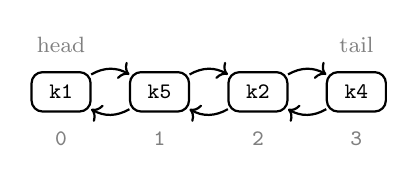
\begin{tikzpicture}

              \node[defaultnode, listnode, scale=0.5] (m1) at (0,0) {};
              \node[defaultnode, listnode, scale=0.5] (m2) at (1.25,0) {};
              \node[defaultnode, listnode, scale=0.5] (m3) at (2.5,0) {};
              \node[defaultnode, listnode, scale=0.5] (m4) at (3.75,0) {};

              \node at (m1) {\footnotesize\texttt{k1}};
              \node at (m2) {\footnotesize\texttt{k5}};
              \node at (m3) {\footnotesize\texttt{k2}};
              \node at (m4) {\footnotesize\texttt{k4}};

              \node[above of =m1, yshift=-4mm, smallgraytext] {head};
              \node[below of =m1, yshift=4mm] {\graytext{\texttt{0}}};
              \node[below of =m2, yshift=4mm] {\graytext{\texttt{1}}};
              \node[below of =m3, yshift=4mm] {\graytext{\texttt{2}}};
              \node[below of =m4, yshift=4mm] {\graytext{\texttt{3}}};
              \node[above of =m4, yshift=-4mm, smallgraytext] {tail};

              \draw[->, thick] (m1) edge[bend left] (m2);
              \draw[->, thick] (m2) edge[bend left] (m3);
              \draw[->, thick] (m3) edge[bend left] (m4);
              \draw[<-, thick] (m1) edge[bend right] (m2);
              \draw[<-, thick] (m2) edge[bend right] (m3);
              \draw[<-, thick] (m3) edge[bend right] (m4);

            \end{tikzpicture}
          \end{figure}
  \end{itemize}
\end{frame}

\begin{frame}
  \begin{itemize}
    \item[(2)] \highlight{\textbf{graphs}} \\
          \graytext{stores pair-wise relationships using vertices and edges}
          \begin{figure}
            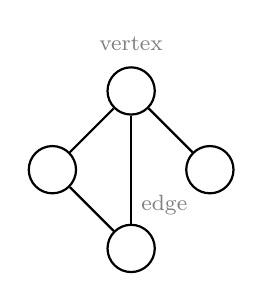
\begin{tikzpicture}
              \tikzset{
                basicnode/.style={
                    shape=circle,
                    draw=black,
                    thick,
                    fill=white,
                    minimum size=6mm,
                    inner sep=0pt
                  }
              }

              \node[basicnode] (m1) at (0,0) {};
              \node[basicnode] (m2) at (-1,-1) {};
              \node[basicnode] (m3) at (1,-1) {};
              \node[basicnode] (m4) at (0,-2) {};

              \node[above of =m1, yshift=-4mm, smallgraytext] {vertex};

              \draw[thick] (m1) edge (m2);
              \draw[thick] (m1) edge (m3);
              \draw[thick] (m1) edge node[right, midway, yshift=-4.5mm, smallgraytext] {edge} (m4);
              \draw[thick] (m2) edge (m4);
            \end{tikzpicture}
          \end{figure}
  \end{itemize}
\end{frame}

\begin{frame}
  \begin{itemize}
    \item[(3)] \highlight{\textbf{trees}} \\
          \graytext{stores hierarchical relationships using vertices and edges, with a single root}\\[3mm]
          \begin{figure}
            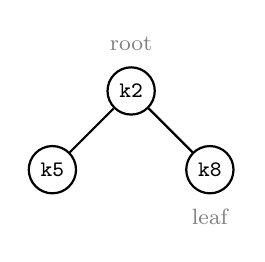
\begin{tikzpicture}

              \tikzset{
                basicnode/.style={
                    shape=circle,
                    draw=black,
                    thick,
                    fill=white,
                    minimum size=6mm,
                    inner sep=0pt
                  }
              }

              \node[basicnode] (m1) at (0,0) {\footnotesize\texttt{k2}};
              \node[basicnode] (m2) at (-1,-1) {\footnotesize\texttt{k5}};
              \node[basicnode] (m3) at (1,-1) {\footnotesize\texttt{k8}};

              \node[above of =m1, yshift=-4mm, smallgraytext] {root};
              \node[below of =m3, yshift=4mm, smallgraytext] {leaf};

              \draw[thick] (m1) edge (m2);
              \draw[thick] (m1) edge (m3);
            \end{tikzpicture}
          \end{figure}
  \end{itemize}
\end{frame}

\begin{frame}
  \begin{itemize}
    \item[(4)] \highlight{\textbf{union-finds}} \\
          \graytext{stores disjoint sets of items representing different groups}
  \end{itemize}
  \begin{figure}
    \centering
    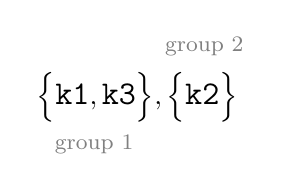
\begin{tikzpicture}
      \node at (0,0.6) {$\Big\lbrace \texttt{\large k1}, \texttt{\large k3} \Big\rbrace,
          \Big\lbrace \texttt{\large k2} \Big\rbrace$};
      \node[smallgraytext] at (-0.55,0) {group 1};
      \node[smallgraytext] at (0.85, 1.25) {group 2};
    \end{tikzpicture}
  \end{figure}
\end{frame}

\begin{frame}
  \begin{itemize}
    \item[(5)] \highlight{\textbf{unordered dictionaries}} \\
          \graytext{stores items by key} \\[3mm]
          \begin{figure}
            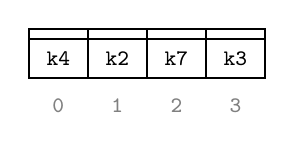
\begin{tikzpicture}

              \tikzset{
                basicnode/.style={
                    shape=rectangle,
                    draw=black,
                    thick,
                    fill=white,
                    minimum width=10mm,
                    minimum height=6mm,
                    inner sep=0pt
                  }
              }
              \coordinate (m1) at (-2.25,0);
              \coordinate (m2) at (-1.5,0);
              \coordinate (m3) at (-0.75,0);
              \coordinate (m4) at (0,0);

              \begin{scope}[scale=0.5, transform shape]
                \pic at (m4) {dictnode={white}};
                \pic at (m3) {dictnode={white}};
                \pic at (m2) {dictnode={white}};
                \pic at (m1) {dictnode={white}};
              \end{scope}

              \node at (m1) {\footnotesize\texttt{k4}};
              \node at (m2) {\footnotesize\texttt{k2}};
              \node at (m3) {\footnotesize\texttt{k7}};
              \node at (m4) {\footnotesize\texttt{k3}};

              \node[draw=white, text=black] (l1) at (-2.25,-0.6) {\footnotesize\graytext{\texttt{0}}};
              \node[draw=white, text=black] (l2) at (-1.5,-0.6) {\footnotesize\graytext{\texttt{1}}};
              \node[draw=white, text=black] (l3) at (-0.75,-0.6) {\footnotesize\graytext{\texttt{2}}};
              \node[draw=white, text=black] (l4) at (0,-0.6) {\footnotesize\graytext{\texttt{3}}};

            \end{tikzpicture}
          \end{figure}
  \end{itemize}
\end{frame}

\begin{frame}
  \begin{itemize}
    \item[(5)] \highlight{\textbf{ordered dictionaries}} \\
          \graytext{stores items in order by key} \\[3mm]
          \begin{figure}
            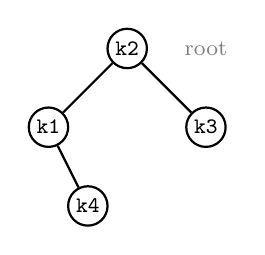
\begin{tikzpicture}

              \node[defaultnode, graphnode] (m1) at (0,0) {\footnotesize\texttt{k2}};
              \node[defaultnode, graphnode] (m2) at (-1,-1) {\footnotesize\texttt{k1}};
              \node[defaultnode, graphnode] (m3) at (1,-1) {\footnotesize\texttt{k3}};
              \node[defaultnode, graphnode] (m4) at (-0.5,-2) {\footnotesize\texttt{k4}};

              \node[right of =m1,xshift=-0mm, smallgraytext] {root};
              \draw[thick] (m1) edge (m2);
              \draw[thick] (m1) edge (m3);
              \draw[thick] (m2) edge (m4);
            \end{tikzpicture}
          \end{figure}
  \end{itemize}
\end{frame}

\begin{frame}
  \begin{itemize}
    \item[(6)] \highlight{\textbf{tries}} \\
          \graytext{stores strings as paths in a tree structure} \\[3mm]
          \begin{figure}
            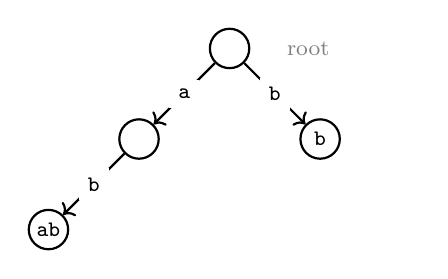
\begin{tikzpicture}

              \node[defaultnode, graphnode] (m1) at (0,0) {$\varnothing$};
              \node[defaultnode, graphnode] (m2) at (-1.15,-1.15) {$\varnothing$};
              \node[defaultnode, graphnode] (m3) at (1.15,-1.15) {\footnotesize\texttt{b}};
              \node[defaultnode, graphnode] (m4) at (-2.3,-2.3) {\footnotesize\texttt{ab}};
              \node (m5) at (2.3,-2.3) {};

              \node[right of =m1, draw=white, xshift=-0mm, smallgraytext] {root};

              \draw[thick, ->] (m1) edge node[midway, fill=white] {\footnotesize \texttt{a}} (m2);
              \draw[thick, ->] (m1) edge node[midway, fill=white] {\footnotesize \texttt{b}} (m3);
              \draw[thick, ->] (m2) edge node[midway, fill=white] {\footnotesize \texttt{b}} (m4);
            \end{tikzpicture}
          \end{figure}
  \end{itemize}
\end{frame}

\begin{frame}
  \begin{itemize}
    \item[(7)] \highlight{\textbf{queues}} \\
          \graytext{stores items in order of priority}\\[2mm]
          \begin{figure}
            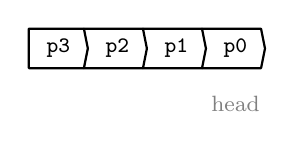
\begin{tikzpicture}

              \coordinate (m1) at (-2.25,0);
              \coordinate (m2) at (-1.5,0);
              \coordinate (m3) at (-0.75,0);
              \coordinate (m4) at (0,0);

              \begin{scope}[scale=0.5, transform shape]
                \pic at (m4) {queuenode={white}};
                \pic at (m3) {queuenode={white}};
                \pic at (m2) {queuenode={white}};
                \pic at (m1) {queuenodetail={white}};
              \end{scope}

              \node at (m1) {\footnotesize\texttt{p3}};
              \node at (m2) {\footnotesize\texttt{p2}};
              \node at (m3) {\footnotesize\texttt{p1}};
              \node at (m4) {\footnotesize\texttt{p0}};

              \node[below of =m4, draw=white, yshift=3mm, width=1cm, smallgraytext] {head};

            \end{tikzpicture}
          \end{figure}
  \end{itemize}
\end{frame}



\begin{frame}{Appendix (Standard Data Structures)}
  \begin{center}
    \Large \highlight{\textbf{appendix}} \\[1mm]
    \normalsize\color{gray} (standard data structures)
  \end{center}
\end{frame}

\begin{frame}[fragile]
  \begin{thmboxtop}
    \highlight{\texttt{List}} \\
    \graytext{(via Doubly Linked Lists)}
    \begin{lstlisting}[style=mypython]
class ListNode:
# attributes    
    # the object of this node
    obj: Object
    
    # the previous node
    prev: Optional[ListNode]
    
    # the next node
    next: Optional[ListNode]
\end{lstlisting}
  \end{thmboxtop}
\end{frame}

\begin{frame}[fragile]
  \begin{thmboxside}
    \begin{lstlisting}[style=mypython, firstnumber=last]
class List:
# attributes:
    # the first node
    head: Optional[ListNode]
    
    # the last node
    tail: Optional[ListNode]
    
    # the number of nodes
    size: Integer
\end{lstlisting}
  \end{thmboxside}
\end{frame}

\begin{frame}[fragile]
  \begin{thmboxbot}
    \begin{lstlisting}[style=mypython, firstnumber=last]
# functions
    # inserts an object before the head
    prepend(obj: Object) -> Optional[Object]
    
    # inserts an object after the tail
    append(obj: Object) -> Optional[ListNode]
    
    # inserts an object after another (if it exists)
    insert(obj: Object, idx: Integer) -> Optional[ListNode]
    
    # returns an object (if it exists)
    get(idx: Integer) -> Optional[ListNode]
    
    # removes an object (if it exists)
    delete(idx: Integer) -> Optional[ListNode]
\end{lstlisting}
  \end{thmboxbot}
\end{frame}


\begin{frame}[fragile]
  \begin{thmboxtop}
    \highlight{\texttt{UnionFind}} \\
    \graytext{(via Binary Forests)}
    \begin{lstlisting}[style=mypython]
class UnifNode:
# attributes
    # the key of this node
    key: Key
    
    # the object of this node
    obj: Object

    # the parent of this node
    pnt: UnifNode
\end{lstlisting}
  \end{thmboxtop}
\end{frame}

\begin{frame}[fragile]
  \vspace{-8mm}
  \begin{thmboxbot}
    \begin{lstlisting}[style=mypython]
class UnionFind:
# attributes
    #  a forest of trees (representing disjoint sets)
    nodes: Dict[Key, UnifNode]
    
    # the number of nodes
    size: Integer

# functions
    # creates a new set for an object
    make_set(key: Key, obj: KeyedObject) -> Optional[UnifNode]
    
    # finds the representative of an object (with path compression)
    find_set(key: Key) -> Optional[UnifNode]

    # unions the representatives two objects (by rank)
    union_sets(key1: Key, key2: Key) -> Optional[UnifNode]
\end{lstlisting}
  \end{thmboxbot}
\end{frame}


\begin{frame}[fragile]
  \begin{thmboxtop}
    \highlight{\texttt{Graph}} \\
    \graytext{(via Adjacency Lists)}
    \begin{lstlisting}[style=mypython]
class Vertex:
# attributes
    # the key of this vertex
    key: Key
    
    # a list of all incoming edges
    in_edges: List[Edge]

    # a list of all outgoing edges
    out_edges: List[Edge]

    # the object of this vertex
    obj: Object
\end{lstlisting}
  \end{thmboxtop}
\end{frame}

\begin{frame}[fragile]
  \begin{thmboxside}
    \begin{lstlisting}[style=mypython, firstnumber=last]
class Edge:
# attributes    
    # the origin of this edge
    from: Vertex
    
    # the destination of this edge
    to: Vertex
    
    # the weight of this edge
    wgt: Integer
\end{lstlisting}
  \end{thmboxside}
\end{frame}

\begin{frame}[fragile]
  \vspace{-6mm}
  \begin{thmboxside}
    \begin{lstlisting}[style=mypython]
class Graph:
# attributes
    # the vertices
    vertices: Dict[Key, Vertex]

    # the edges
    edges: List[Edge]

# functions
    # adds/updates a vertex
    insert_vertex(key: Key, obj: Object: Object) -> Optional[Vertex]
    
    # adds/updates an edge from two vertices (if they exist)
    insert_edge(key1: Key, key2: Key, wgt: Integer) -> Optional[Edge]

    ...
\end{lstlisting}
  \end{thmboxside}
\end{frame}

\begin{frame}[fragile]
  \vspace{-9mm}
  \begin{thmboxbot}
    \begin{lstlisting}[style=mypython, firstnumber=last]
    # returns a vertex (if it exists)
    get_vertex(key: Key) -> Optional[Vertex]

    # returns all vertices
    get_vertices() -> List[Vertex]
    
    # returns all edges from one vertex to another
    get_edges_btw(key: Key, obj: Object: Object) -> Optional[Vertex]
    
    # returns all edges from a vertex
    get_edges_from(key: Key) -> List[Edge]

    # returns all edges to a vertex
    get_edges_to(key: Key) -> List[Edge]

    # returns all edges
    get_edges() -> List[Edge]
\end{lstlisting}
  \end{thmboxbot}
\end{frame}

\begin{frame}[fragile]
  \begin{thmboxtop}
    \highlight{\texttt{Dict}} \\
    \graytext{(via Hash Tables)}
    \begin{lstlisting}[style=mypython]
class DictNode:
# attributes
    # the key of this node
    key: Key

    # the keyed object of this node
    obj: Object
\end{lstlisting}
  \end{thmboxtop}
\end{frame}

\begin{frame}[fragile]
  \vspace{-8mm}
  \begin{thmboxside}
    \begin{lstlisting}[style=mypython]
class Dict:
# attributes
    # an array of items
    buckets: Array[List[DictNode]]
    
    # a hash function
    hash_fnc: Function[[Key], [Integer]]

    # a probe function
    probe_fnc: Function[[Integer], [Integer]]
    
    # the number of nodes in the array (excluding chaining)
    size: Integer

    # the number of spots in the array
    capacity: Integer
\end{lstlisting}
  \end{thmboxside}
\end{frame}

\begin{frame}[fragile]
  \begin{thmboxbot}
    \begin{lstlisting}[style=mypython]
# functions
    # inserts/updates an object
    insert(key: Key, obj: Object: Object) -> Optional[DictNode]

    # returns an object (if it exists)
    get(key: Key) -> Optional[DictNode]

    # removes an object (if it exists)
    delete(key: Key) -> Optional[DictNode]
\end{lstlisting}
  \end{thmboxbot}
\end{frame}

\begin{frame}[fragile]
  \vspace{-10mm}
  \begin{thmboxtop}
    \highlight{\texttt{Trie}} \\
    \graytext{(via Trees)}
    \begin{lstlisting}[style=mypython]
class TrieNode:
# attributes
    # the object of this node
    obj: Optional[Object]

    # the children of this node
    children: Dict[Key, TrieNode]

    # the parent of this node
    pnt: Optional[TrieNode]
\end{lstlisting}
  \end{thmboxtop}
\end{frame}

\begin{frame}[fragile]
  \vspace{-5mm}
  \begin{thmboxbot}
    \begin{lstlisting}[style=mypython]
class Trie:
# attributes
    # the root
    root: TrieNode

# functions
    # inserts an object, creating nodes for each character as needed
    insert(key: Key, obj: Object) -> Optional[TrieNode]

    # returns the closest prefix match
    get(key: Key) -> Optional[TrieNode]

    # removes an object (if it exists) and any extra nodes
    delete(key: Key) -> Optional[TrieNode]
\end{lstlisting}
  \end{thmboxbot}
\end{frame}


\begin{frame}[fragile]
  \begin{thmboxtop}
    \highlight{\texttt{Tree}} \\
    \graytext{(via Adjacency Lists)}
    \begin{lstlisting}[style=mypython]
class TreeNode:
# attributes
    # the key of this node
    key: Key
    
    # the object of this node
    obj: Object

    # the children of this node 
    children: List[TreeNode]

    # the parent of this node
    pnt: Optional[TreeNode]
\end{lstlisting}
  \end{thmboxtop}
\end{frame}

\begin{frame}[fragile]
  \vspace{-5mm}
  \begin{thmboxtop}
    \begin{lstlisting}[style=mypython]
class Tree:
# attributes
    # the root
    root: Optional[TreeNode]

    # the number of vertices
    size: Integer

# functions
    # adds/update an object as a child another (if it exists)
    append_vertex(key: Key, obj: Object, pos: Key) -> Optional[TreeNode]

    # returns an object (if it exists)
    get_vertex(key: Key) -> Optional[TreeNode]

    # delete an object if it exists and is a leaf
    delete_vertex(key: Key) -> Optional[TreeNode]
\end{lstlisting}
  \end{thmboxtop}
\end{frame}

\begin{frame}[fragile]
  \vspace{-10mm}
  \begin{thmboxtop}
    \highlight{\texttt{Ordict}} \\
    \graytext{(via Balanced Binary Search Trees)}
    \begin{lstlisting}[style=mypython]
class OrdictNode:
# attributes
    # the key of this node
    key: Key

    # the object of this node
    obj: Object

    # the left child of this node
    left: Optional[OrdictNode]

    # the right child of this node
    right: Optional[OrdictNode]

    # the parent of this node
    pnt: Optional[OrdictNode]
\end{lstlisting}
  \end{thmboxtop}
\end{frame}

\begin{frame}[fragile]
  \vspace{-5mm}
  \begin{thmboxbot}
    \begin{lstlisting}[style=mypython]
class Ordict:
# attributes
    # the root
    root: Optional[OrdictNode]
    
    # the number of nodes
    size: Integer
    
# functions
    # inserts/updates an object
    insert(key: Key, obj: Object) -> Optional[OrdictNode]

    # returns an object (if it exists)
    get(key: Key) -> Optional[OrdictNode]

    # removes an object (if it exists)
    delete(key: Key) -> Optional[OrdictNode]
\end{lstlisting}
  \end{thmboxbot}
\end{frame}

\begin{frame}[fragile]
  \begin{thmboxtop}
    \highlight{\texttt{Queue}} \\
    \graytext{via Heaps}
    \begin{lstlisting}[style=mypython]
class QueueNode:
# attributes
    # the object of this node
    obj: Object

    # the priority of this node
    pri: Integer
\end{lstlisting}
  \end{thmboxtop}
\end{frame}

\begin{frame}[fragile]
  \begin{thmboxbot}
    \begin{lstlisting}[style=mypython]
class Queue:
# attributes
    # the array representing the underlying heap
    arr: Array[QueueNode]

# functions
    # inserts an object with a priority of pri
    push(obj: Object, pri) -> Optional[QueueNode]

    # removes and returns the object with the maximum/minimum priority  
    pop() -> Optional[QueueNode]

    # returns the object with the maximum/minimum priority
    peak() -> Optional[QueueNode]
\end{lstlisting}
  \end{thmboxbot}
\end{frame}

\end{document}